\section{Design}\label{sec:design}

\subsection{Overview}\label{sec:design_overview}

The system features a virtual environment in which the user sees themselves
driving a car. The controls of the car are wired up to a remote car actually
driving around with a camera. Additionally, the user is equipped with a GSR
sensor, and their stress level is used to determine the speed of the vehicle.

\subsection{Breakdown into Systems}\label{sec:design_systems}

The system was broken down into multiple independent systems (Please refer to
Figure~\ref{fig:systems} for a big-picture overview of the systems involved),

\begin{itemize}
\item Stress detection system (Described in Section~\ref{sec:design_system_stress})%
\item Arduino car control system (Described in
Section~\ref{sec:design_arduino})%
\item Socket server (Described in Section~\ref{sec:design_socket_server})
\item VR Enviroment (Described in Section~\ref{sec:design_vr_enviroment})
  % TODO: List all the systems
\item Camera Livestream (Described in Section~\ref{sec:design_camera_livestream})

\begin{figure*}
  \centering
  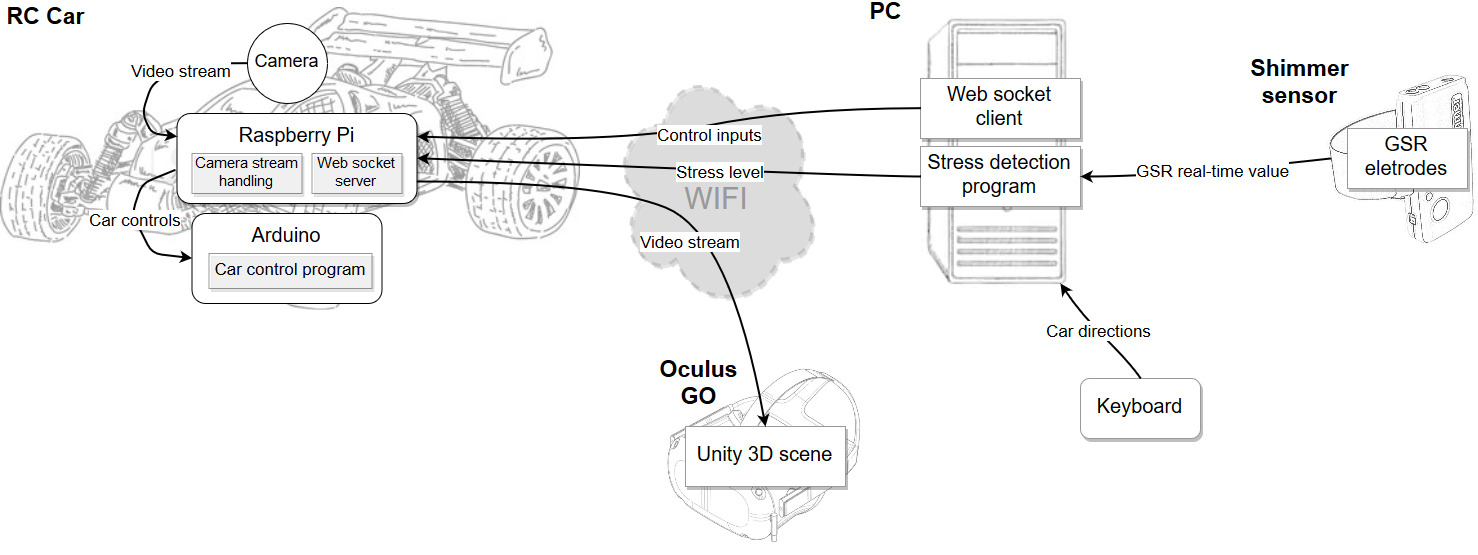
\includegraphics[width=\textwidth]{system_design_scheme/system_design_sketch.jpg}
  \caption{\label{fig:systems} A big-picture overview of the systems
  involved.}
\end{figure*}

\end{itemize}

\subsection{Stress detection system}\label{sec:design_system_stress}

The goal of the stress detection subsystem was to output the user's stress
level from the data collected by the physiological sensors. Based on the
Shimmer3 GSR+ Unit, the system uses finger GSR electrodes feeding the sensors'
central unit with real-time GSR data. The HR was abandoned due to several
reasons: a lag in HR response compared to GSR response leading to a gap
between points of data that would demonstrate some stress state, too much
variability and a low reliability on the collected data and a rate of failure
that would have meant that the data needed to be corrected continuously and
induce too important initialization delays. The analysis and computations
on the data were done on a computer so the data was sent via Bluetooth from
the Shimmer wearable unit to the computer.

The main program was written in C\# since Shimmer provides a C\# API to
communicate with its sensors.  The idea behind the main stress detection
program is using every second GSR data to find clusters in the data and
defining classes and then assign each a corresponding level of stress which,
then, will be sent to the car control system. To do so, after an initialization
delay, the GSR data is collected every second for a certain amount of time.
After that, a k-means algorithm is run over the collected data to compute
the user GSR-stress profile (as user GSR variability is one of the main
concerns). Then, each new point of data is assigned to the closest cluster
mean (output by the k-means algorithm) with respect to Euclidean distance. It
was decided to do so after finding out that running a k-means every second
would be too computational expensive.

After this first step, the program is running in and endless mode, computing
new clusters regularly since it had been observed that Skin resistance mean
tend to decrease slowly over time before stabilizing. Another point of doing
so is that it will allow the algorithm to adapt to the moment, and especially,
it will adapt its stress levels to the ones experienced within the last n
(delay between two k-means runs) minutes, making it more or less sensitive
to stress state changing depending on the previous measurements. The output
is communicated to the car control system through WiFi.

Tweaking the initialization delay parameter only has the minor effect
of delaying more or less the starting time for collecting GSR data while
changing the k-means delay will have a relevant impact on the system. On one
hand, a longer k-means delay will force the algorithm to wait for more time
and collect more data before computing new clusters. As an effect, it will
build a more ``user-close'' profile and will be less prone to overreaction
(between stress levels causing change from one to another too often) and
misclassification (mistake on stress level affection) but it will inevitably
be less reactive and adaptive. On the other hand, setting a shorter k-means
delay will lead to the building of a more ``moment-close'' profile, more
reactive and representative of the current stress level of the driver.

A balance has to be found, depending on what the user wants and on the type
of activity that is being monitored. For example, a real-world drive lasts
longer than a simulated one, which allows for longer time to collect data.
Additionally, stressors (potentially stressful events) don't come at the same
rate and with the same impact in the simulated scenario as the real-world
one. The number of stress levels corresponds to the number of clusters built
by the algorithm. It was determined that 3 was a relevant choice for this
parameter. Although the algorithm works well for most numbers, it has
more to do with want to do with this output and how much data is collected
between each clusterization. In the case of the project, only a few levels
were needed to affect the speed of a car in a noticeable way (not too slight).

\subsection{Arduino car control system}\label{sec:design_arduino}

The remote-controlled car used in the project had only been used for autonomous
driving training, so its internal code had to be adapted for external
control. This was accomplished using the following set of state variables,

\begin{itemize}
  \item \mintinline{cpp}{throttleState} --- Responsible for propulsion
    direction. Default state: S
    
    Possible states: [(F)orward, (S)tationary, (B)ackward]
  \item \mintinline{cpp}{steeringState} --- Responsible for the angle of the
    wheels. Default state: C
    
    Possible states: [(L)eft, (C)enter, (R)ight]
  \item \mintinline{cpp}{stressState} --- An indicator of driver stress
  level. Responsible for velocity, where a lower stress resulted in a higher
  velocity. Default state: 2
    
    Possible states: [1 Low, 2 Medium, 3 High]
\end{itemize}

The state variables were set by sending single bytes of instructions to its
serial port, which in turn determined what signals were sent to the functions
controlling the car.  This design facilitated decoupling of the imperative
serial signals from the control system of the car. It could thus be programmed
to return to a standstill when no throttle commands had been received for
an appropriate time interval, to ensure safety in the case of a broken signal.

\subsection{Socket Server}\label{sec:design_socket_server}

The Arduino board did not have any networking capabilities, which worked for
the car's original design for autonomous driving. It was decided that the
simplest way to add such support would be to attach a Raspberry Pi (which
has networking capabilities) to the car, and to let it forward the signals
to the Arduino board via it's serial port.

The distributed nature of the system meant that the Raspberry Pi would have
to handle socket connections to multiple devices and let them pass messages
to the Arduino simultaneously.

In terms of implementation, this meant hosting two separate socket servers.
One for driving, and one for stress levels of the driver. The socket servers
supported the following messages.

\begin{itemize}
  \item \mintinline{cpp}{up} --- Drive the car forward
  \item \mintinline{cpp}{right} --- Steer the wheels to the right
  \item \mintinline{cpp}{down} --- Stop or drive the car backwards
  \item \mintinline{cpp}{left} --- Steer the wheels to the left
  \item \mintinline{cpp}{low} --- Low stress level
  \item \mintinline{cpp}{medium} --- Medium stress level
  \item \mintinline{cpp}{high} --- High stress level
\end{itemize}

These messages are stored directly in a queue, which is then handled by a
separate thread, and is responsible for handling these messages and deciding
what messages to send to the Arduino over the serial port.


\subsection{VR Environment}\label{sec:design_vr_enviroment}

In order to induce a real driving sensation to the user, a VR environment was
generated with Unity, working in the Oculus GO device. In this environment,
the user finds themselves inside a car. Through the back, left and right
windows of the virtual car, the user can see a further street environment. In
the front window, the user will find the view provided by the Pi camera.

Oculus GO has only 3 degrees of freedom (pitch, yaw, roll), so it is not
necessary generating a full car and street model. The user is only able to
see from a strict point in the VR space. So, the car and the street have been
generated with 2 different spheres, and applying 3D images as textures. The
user can look in any direction, and they will see a consistent world.

In front of the virtual car, there is a screen. This screen is only visible
from the front window of the car, so the user has a sensation of being driving
the Arduino car. The image shown in the screen is loaded from the server,
and updated each frame in the VR environment.

A picture of the environment can be found in Figure~\ref{fig:environment} and a
picture from the inside of the car can be found in Figure~\ref{fig:inside_car}.

\begin{figure}[H]
  \centering 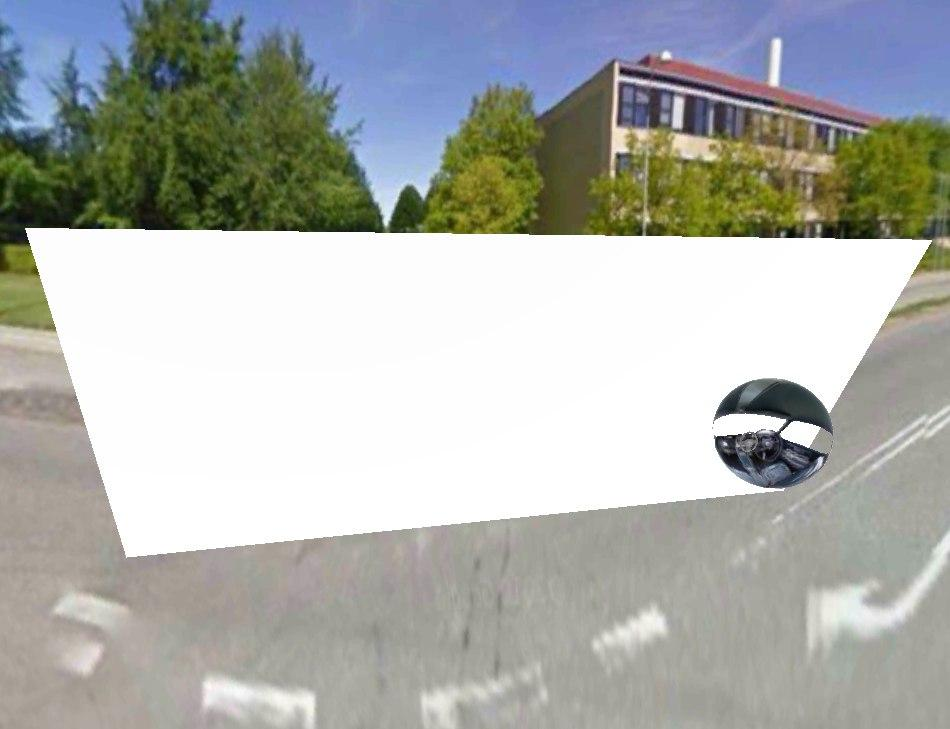
\includegraphics[width=\textwidth / 2]{./screen.jpg}
  \caption{\label{fig:environment} The environment around the car. The white
  box is where the car will be.}
\end{figure}

\begin{figure}[H]
  \centering 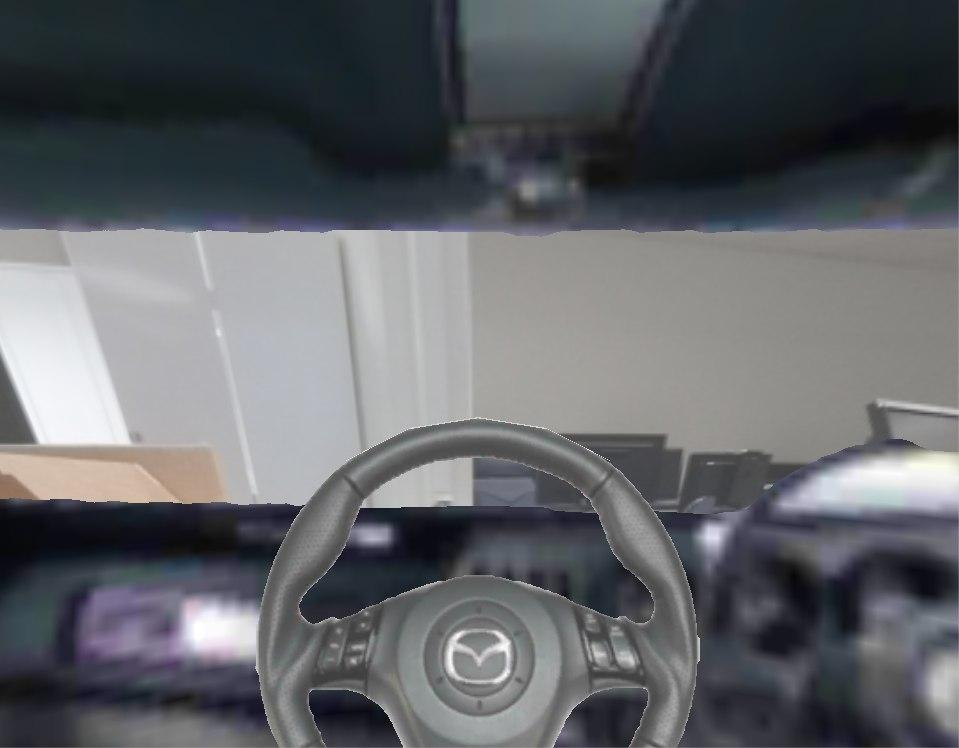
\includegraphics[width=\textwidth / 2]{./inside_car.jpg}
  \caption{\label{fig:inside_car} The view from inside the car.}
\end{figure}


\subsection{Camera Livestream}\label{sec:design_camera_livestream}

If the VR Environment is going to be useful, a live camera feed has to be given
so that you can see where you're driving. This is done using the Raspberry Pi
along with it's camera attachment.

A very simple HTTP server was written in Python, with the sole purpose of
sending the camera stream. HTTP was chosen because of the need to input the video stream into the virtual environement that was built with Unity which natively supports HTTP video streams. The PiCamera library \cite{picamera} is used to
access the camera feed within Python, which is then streamed as mjpeg over the
HTTP server.

The camera supports recording up to 1080p, however due to hardware limitations
on the Raspberry Pi, WiFi router and Oculus Go, it was decided to use a
low resolution (400x200) for the camera feed. Any higher resolutions would
lead the video stream being uneven and suffering frequent delays.  A high
frame-rate is necessary for the best possible immersion, so 60 Frames Per
Second camera feed is used.
